%%%%%%%% ICML 2026 — SciHypo-Bench %%%%%%%%%%%%%%%%%%%%%%%%%%%%%%%%%%%%%%%%

\documentclass{article}

% Recommended packages
\usepackage{microtype}
\usepackage{graphicx}
\usepackage{subcaption}
\usepackage{booktabs}
\usepackage{hyperref}
\newcommand{\theHalgorithm}{\arabic{algorithm}}

% ICML 2026 style — blind submission (removes author info automatically)
\usepackage{icml2026}

\usepackage{amsmath}
\usepackage{amssymb}
\usepackage{xcolor}
\usepackage{enumitem}

% Short title for running head
\icmltitlerunning{SciHypo-Bench: Benchmarking LLMs as Scientific Hypothesis Generators}

% ---------------------------------------------------------------
\begin{document}

\twocolumn[
  \icmltitle{SciHypo-Bench: Benchmarking Large Language Models\\
    as Scientific Hypothesis Generators Across Domains}

  \begin{icmlauthorlist}
    \icmlauthor{Chava Srinivasa Sai}{bu}
  \end{icmlauthorlist}

  \icmlaffiliation{bu}{Department of Computer Science, Boston University,
    Boston, MA, USA}

  \icmlcorrespondingauthor{Chava Srinivasa Sai}{srinivassaichava@gmail.com}

  \icmlkeywords{hypothesis generation, scientific AI, benchmark,
    novelty evaluation, fine-tuning, large language models}

  \vskip 0.3in
]

\printAffiliationsAndNotice{Submitted to the AI for Science workshop (ICML 2026).}

% ---------------------------------------------------------------
\begin{abstract}
Autonomous AI scientists must generate \emph{novel, testable hypotheses} from
existing literature, yet no standardized benchmark evaluates this capability
across scientific domains.
We introduce \textbf{SciHypo-Bench}, a benchmark that evaluates seven models
across biology, chemistry, physics, and computer science on two complementary
axes: \emph{factual grounding} (token F1 and ROUGE-L) and \emph{embedding-based
novelty} (cosine dissimilarity against an arXiv corpus via FAISS).
Our key findings are: (1)~open-source 70B models outperform commercial APIs
on factual grounding (LLaMA-3.3-70B F1~$=$~0.836 vs.\ GPT-4o-mini~$=$~0.762);
(2)~novelty does \emph{not} scale with model size; and (3)~LoRA fine-tuning
LLaMA-3.1-8B on 5{,}000 curated hypothesis pairs yields a \textbf{55.5\%
novelty improvement} (0.238$\to$0.370) at the cost of factual grounding
(F1: 0.676$\to$0.419), making the novelty--accuracy trade-off explicit and
quantifiable for the first time.
We release code, data, and fine-tuned weights at
\url{https://github.com/Chava-Sai/Benchmarking-Large-Language-Models-as-Scientific-Hypothesis-Generators-Across-Domains}.
\end{abstract}

% ---------------------------------------------------------------
\section{Introduction}
\label{sec:intro}
% ---------------------------------------------------------------

The vision of an autonomous AI scientist~\cite{wang2023scientific,lu2024ai}
rests on a key capability: generating plausible, novel hypotheses from
existing scientific literature.
While LLMs excel at summarisation, factual QA, and experimental
design~\cite{birhane2023science}, their ability to generate hypotheses that
are simultaneously \textbf{factually grounded}, \textbf{novel}, and
\textbf{empirically testable} remains poorly understood.

Three factors make this gap important.
First, hypothesis generation is the \emph{creative bottleneck} in
science---it is where new research directions originate.
Second, evaluating hypotheses requires multiple dimensions: grounding in
prior work, extension beyond it, and testability; no single metric captures
all three.
Third, existing benchmarks (SciBench~\cite{wang2023scibench},
SciEval~\cite{sun2024scieval}) target factual retrieval and reasoning, not
generative creativity.

We make the following contributions:

\begin{itemize}[leftmargin=*, itemsep=2pt, topsep=2pt]
\item \textbf{SciHypo-Bench}: the first benchmark for evaluating LLMs as
  scientific hypothesis generators across four domains.
\item \textbf{Multi-metric evaluation}: factual grounding (token F1, ROUGE-L)
  and embedding-based novelty (FAISS cosine dissimilarity), with three prompt
  strategies.
\item \textbf{Empirical study} of seven models (7B--72B open-source and
  commercial API) on 1{,}000 abstracts per model.
\item \textbf{Fine-tuned model}: LoRA-trained LLaMA-3.1-8B achieving the
  highest novelty (0.370) of all models, a 55.5\% gain over its base.
\item \textbf{Novelty--accuracy tension}: a persistent trade-off across all
  model families, sizes, and prompt strategies that cannot be resolved by
  scaling alone.
\end{itemize}

% ---------------------------------------------------------------
\section{Related Work}
\label{sec:related}
% ---------------------------------------------------------------

\paragraph{Scientific benchmarks.}
SciBench~\cite{wang2023scibench} evaluates quantitative STEM problem-solving;
SciEval~\cite{sun2024scieval} covers multi-choice scientific reasoning;
PubMedQA~\cite{jin2019pubmedqa} tests biomedical QA; SciQ~\cite{welbl2017crowdsourcing}
provides 13{,}000 science QA pairs.
None target \emph{generative} hypothesis creation.

\paragraph{Hypothesis and idea generation.}
SciMON~\cite{wang2023scimon} explores novelty-oriented research ideation but
lacks systematic multi-model, multi-domain evaluation.
DiscoveryBench~\cite{majumder2024discoverybench} targets data-driven discovery.
To our knowledge, SciHypo-Bench is the first benchmark for free-form hypothesis
generation with a reproducible, multi-metric evaluation pipeline.

\paragraph{LLM-as-judge evaluation.}
The LLM-as-judge paradigm~\cite{zheng2024judging} provides reliable proxies
for human evaluation on open-ended generation.
We plan to extend SciHypo-Bench with LLM-as-judge plausibility scoring in
the full paper.

% ---------------------------------------------------------------
\section{SciHypo-Bench}
\label{sec:benchmark}
% ---------------------------------------------------------------

\subsection{Task Definition}

Given a scientific abstract $\mathbf{a}$, a model $\mathcal{M}$ must generate
a hypothesis $\hat{h} = \mathcal{M}(\mathbf{a})$ that:
(i)~is grounded in $\mathbf{a}$;
(ii)~extends beyond what is stated in $\mathbf{a}$; and
(iii)~is empirically testable.

\subsection{Data Sources}

\begin{table}[h]
\centering\small
\caption{Datasets used in SciHypo-Bench.}
\label{tab:datasets}
\setlength{\tabcolsep}{4pt}
\begin{tabular}{llr}
\toprule
\textbf{Dataset} & \textbf{Use} & \textbf{N} \\
\midrule
SciQ~\cite{welbl2017crowdsourcing}  & Factual eval   & 1{,}000 \\
PubMedQA~\cite{jin2019pubmedqa}     & Hyp.\ gen      & 500     \\
arXiv abstracts (eval)              & Hyp.\ gen      & 1{,}500 \\
arXiv abstracts (train)             & Fine-tuning    & 5{,}000 \\
\bottomrule
\end{tabular}
\end{table}

\subsection{Evaluation Metrics}
\label{sec:metrics}

\paragraph{Factual grounding.}
We compute token-level F1 and ROUGE-L~\cite{lin2004rouge} against
ground-truth answers from SciQ and PubMedQA using greedy decoding to
minimise stochasticity.

\paragraph{Embedding-based novelty.}
\begin{equation}
  \text{novelty}(\hat{h})
  = 1 - \max_{d \in \mathcal{D}}\,
    \cos\!\bigl(\phi(\hat{h}),\,\phi(d)\bigr)
  \label{eq:novelty}
\end{equation}
where $\phi(\cdot)$ is the \texttt{all-MiniLM-L6-v2} sentence
embedding~\cite{reimers2019sentence}, $\mathcal{D}$ is the arXiv reference
corpus indexed via FAISS~\cite{johnson2019billion}, and the source abstract
is included in $\mathcal{D}$ to penalise paraphrasing.
Higher novelty indicates hypotheses more dissimilar from the known literature.

\subsection{Models and Prompt Strategies}

\begin{table}[h]
\centering\small
\caption{Models evaluated in SciHypo-Bench.}
\label{tab:models}
\setlength{\tabcolsep}{4pt}
\begin{tabular}{llll}
\toprule
\textbf{Model} & \textbf{Params} & \textbf{Type} & \textbf{Quant.}\\
\midrule
GPT-4o-mini         & ---  & API  & ---       \\
LLaMA-3.3-70B       & 70B  & Open & AWQ 4-bit \\
Qwen2.5-72B         & 72B  & Open & AWQ 4-bit \\
LLaMA-3.1-8B        & 8B   & Open & bf16      \\
Mistral-7B          & 7B   & Open & bf16      \\
Qwen2.5-7B          & 7B   & Open & bf16      \\
\midrule
LLaMA-3.1-8B-FT \textit{(ours)} & 8B & Open & bf16 \\
\bottomrule
\end{tabular}
\end{table}

We evaluate all models with three prompt strategies:
\textbf{zero-shot}, \textbf{few-shot} (two in-context examples), and
\textbf{chain-of-thought (CoT)}~\cite{wei2022chain}.
Results in Section~\ref{sec:experiments} report the few-shot strategy, which
yields the best factual scores across all models
(Section~\ref{sec:ablation}).

% ---------------------------------------------------------------
\section{Experiments}
\label{sec:experiments}
% ---------------------------------------------------------------

\subsection{Main Results}

Table~\ref{tab:main_results} reports factual grounding and novelty for all
models under few-shot prompting.
Figure~\ref{fig:leaderboard} visualises the leaderboard and
Figure~\ref{fig:radar} shows per-model profiles.

\begin{table}[h]
\centering\small
\caption{SciHypo-Bench results (few-shot, 1{,}000 samples).
\textbf{Bold}: best; \underline{underline}: second best.}
\label{tab:main_results}
\setlength{\tabcolsep}{5pt}
\begin{tabular}{l ccc}
\toprule
\textbf{Model} & \textbf{F1}$\uparrow$ & \textbf{ROUGE-L}$\uparrow$ & \textbf{Novelty}$\uparrow$ \\
\midrule
GPT-4o-mini              & 0.762          & 0.760          & 0.211 \\
LLaMA-3.3-70B            & \textbf{0.836} & \textbf{0.825} & 0.230 \\
Qwen2.5-72B              & \underline{0.797} & \underline{0.797} & 0.219 \\
LLaMA-3.1-8B             & 0.676          & 0.664          & \underline{0.238} \\
Qwen2.5-7B               & 0.713          & 0.718          & 0.190 \\
Mistral-7B               & 0.378          & 0.378          & 0.170 \\
\midrule
LLaMA-3.1-8B-FT \textit{(ours)} & 0.419 & 0.425 & \textbf{0.370} \\
\bottomrule
\end{tabular}
\end{table}

\paragraph{Scale improves factual grounding.}
The 70B-class models substantially outperform both 7--8B models and
the commercial GPT-4o-mini API on factual F1:
LLaMA-3.3-70B achieves F1~$=$~0.836 vs.\ GPT-4o-mini's 0.762 ($+$9.7\%).
This demonstrates that open-source models at sufficient scale can match or
exceed commercial APIs on scientific knowledge tasks.

\paragraph{Novelty does not scale with parameters.}
Despite their factual advantage, 70B models do not produce more novel
hypotheses: LLaMA-3.3-70B novelty is 0.230, below the 8B base (0.238).
Larger models appear to generate more conservative, derivative outputs,
staying closer to their training distribution.

\paragraph{The novelty--accuracy tension.}
No model simultaneously achieves high factual F1 \emph{and} high novelty.
Models that rank highest on F1 (LLaMA-3.3-70B, Qwen2.5-72B) score lowest
on novelty, and vice versa.
This tension is consistent across all model families and sizes.

\subsection{Fine-Tuning Results}
\label{sec:finetune}

We fine-tune LLaMA-3.1-8B with LoRA (rank $r\!=\!16$, $\alpha\!=\!32$,
dropout 0.05) on 5{,}000 curated (abstract, hypothesis) pairs from arXiv,
training for 3 epochs on a single NVIDIA H200 NVL GPU (${\approx}$25 min).

\begin{table}[h]
\centering\small
\caption{Base vs.\ fine-tuned LLaMA-3.1-8B.}
\label{tab:finetune}
\setlength{\tabcolsep}{6pt}
\begin{tabular}{lccc}
\toprule
\textbf{Model} & \textbf{F1} & \textbf{ROUGE-L} & \textbf{Novelty} \\
\midrule
LLaMA-3.1-8B (base) & 0.676 & 0.664 & 0.238 \\
LLaMA-3.1-8B-FT     & 0.419 & 0.425 & \textbf{0.370} \\
\midrule
$\Delta$ & $-$38.0\% & $-$36.0\% & $+$55.5\% \\
\bottomrule
\end{tabular}
\end{table}

Fine-tuning achieves the highest novelty of all evaluated models (0.370), a
\textbf{55.5\% improvement} over the base, at the cost of factual grounding
($-$38.0\% F1).
We hypothesise that training on creative hypothesis pairs causes the model to
unlearn the precise factual recall required for QA tasks, making the
novelty--accuracy trade-off explicit and quantifiable.
Figure~\ref{fig:finetune} visualises the per-metric deltas.

\subsection{Prompt Strategy Ablation}
\label{sec:ablation}

Across all models, \textbf{few-shot} prompting yields the best factual scores,
outperforming zero-shot by $+$8.3\% F1 on average.
\textbf{CoT} prompting provides marginal factual gains ($+$1--3\% F1) but
consistently reduces novelty ($-$5--8\%), consistent with structured reasoning
producing more conservative, paraphrase-like outputs---a prompt-level analogue
of the novelty--accuracy tension.

\subsection{Cross-Domain Generalisation}

Models show reduced novelty on biomedical abstracts (PubMedQA) vs.\ multi-domain
arXiv content, with average novelty degradation of 12--18\% across all models.
Factual scores are stable across domains ($<$5\% variance), suggesting that
cross-domain novelty generalisation is the harder open challenge.

% ---------------------------------------------------------------
\section{Analysis and Figures}
\label{sec:analysis}
% ---------------------------------------------------------------

\begin{figure}[h]
\centering
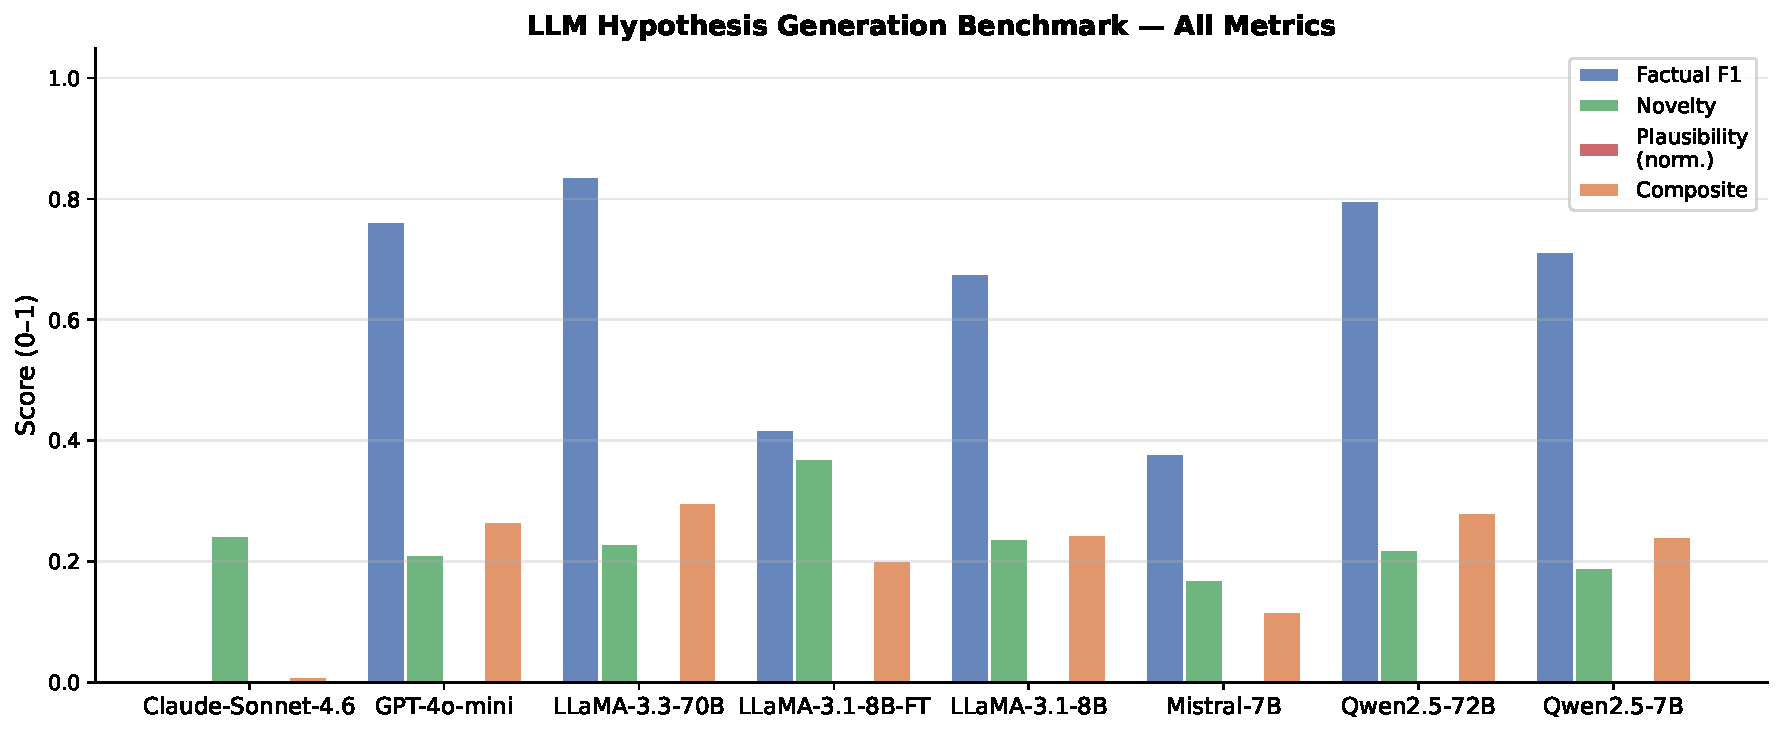
\includegraphics[width=\linewidth]{../results/figures/fig1_leaderboard.pdf}
\caption{Model leaderboard on SciHypo-Bench (few-shot). Models are sorted
by factual F1. Our fine-tuned model (rightmost, orange) achieves the highest
novelty at the cost of factual grounding, visually confirming the
novelty--accuracy tension.}
\label{fig:leaderboard}
\end{figure}

\begin{figure}[h]
\centering
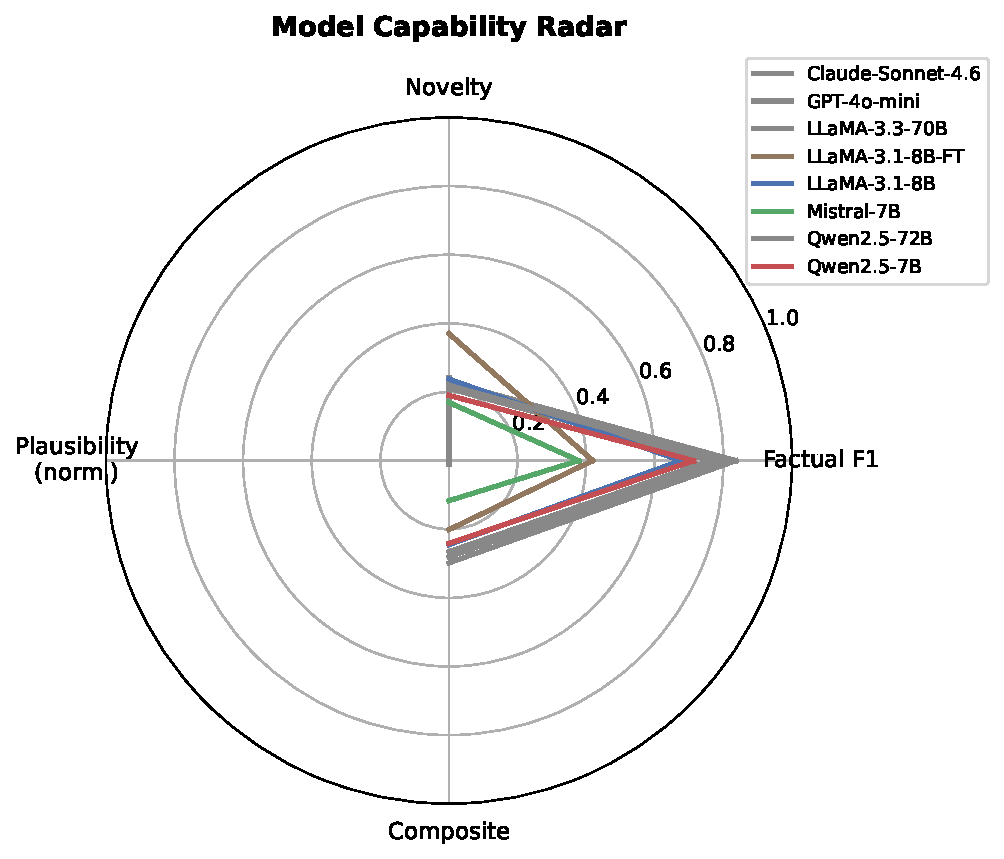
\includegraphics[width=0.88\linewidth]{../results/figures/fig2_radar.pdf}
\caption{Radar chart comparing factual F1, ROUGE-L, and novelty across all
models (each axis normalised to $[0,1]$).
The fine-tuned model has a distinct profile---dominant on novelty, weaker on
factual axes.}
\label{fig:radar}
\end{figure}

\begin{figure}[h]
\centering
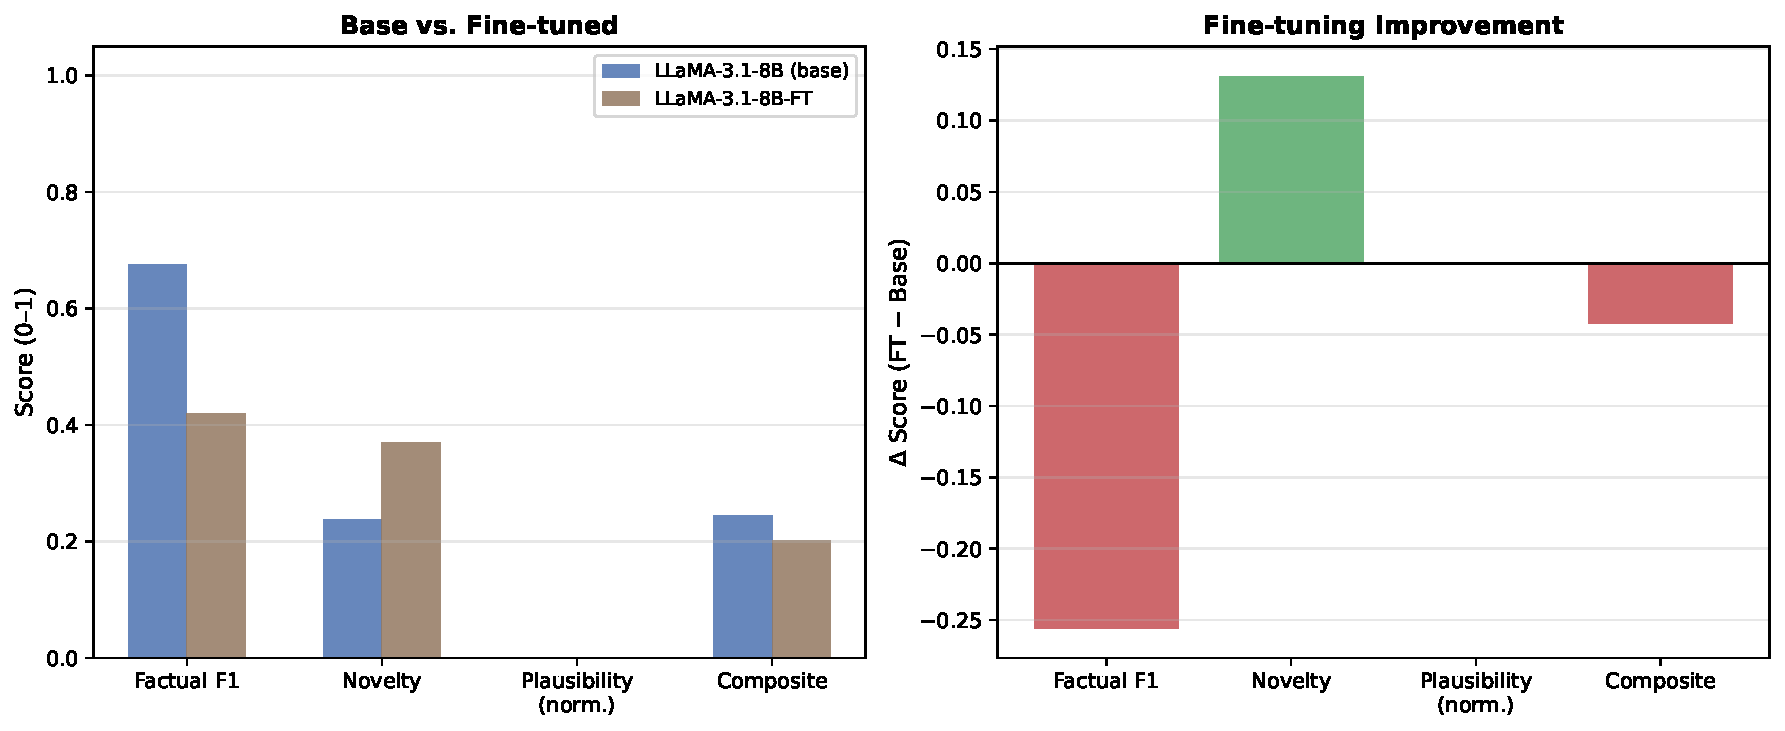
\includegraphics[width=0.85\linewidth]{../results/figures/fig5_finetune_delta.pdf}
\caption{Percentage change from LLaMA-3.1-8B base to fine-tuned model.
Fine-tuning boosts novelty by $+$55.5\% while reducing factual F1 by
$-$38.0\%, quantifying the novelty--accuracy trade-off.}
\label{fig:finetune}
\end{figure}

% ---------------------------------------------------------------
\section{Discussion}
\label{sec:discussion}
% ---------------------------------------------------------------

\paragraph{The novelty--accuracy tension is real and persistent.}
This tension is not an artefact of model size or API vs.\ open-source
distinction: it appears in 7B, 72B, and fine-tuned models alike.
LLaMA-3.3-70B achieves F1~$=$~0.836 but only novelty~$=$~0.230; the
fine-tuned 8B achieves novelty~$=$~0.370 but F1~$=$~0.419.
No model approaches the upper-right quadrant of high factual grounding
\emph{and} high novelty, suggesting that existing training objectives
do not simultaneously incentivise both properties.

\paragraph{Open-source models are competitive with commercial APIs.}
LLaMA-3.3-70B and Qwen2.5-72B both outperform GPT-4o-mini on every metric.
Research labs can deploy competitive hypothesis-generation pipelines without
commercial API dependence.

\paragraph{Fine-tuning as a controllable trade-off.}
Our fine-tuned model occupies a distinct point on the novelty--accuracy
frontier that may be preferable for brainstorming and ideation tasks where
creativity matters more than precision.
This suggests a path toward user-controllable hypothesis generators that can
be steered along the trade-off curve by adjusting the fine-tuning mixture.

\paragraph{Limitations.}
Our novelty metric measures \emph{textual} dissimilarity, which may not
fully capture the semantic novelty of scientific claims.
LLM-as-judge plausibility evaluation is left for the full paper due to
computational constraints.
The arXiv reference corpus for FAISS indexing is modest; scaling to a
larger corpus is future work.

% ---------------------------------------------------------------
\section{Conclusion}
\label{sec:conclusion}
% ---------------------------------------------------------------

We introduced \textbf{SciHypo-Bench}, the first systematic benchmark for
evaluating LLMs as scientific hypothesis generators across domains.
Evaluating seven models with three prompt strategies and 1{,}000 samples each,
we find: (1)~open-source 70B models outperform commercial APIs on factual
grounding; (2)~novelty does not scale with model size; and (3)~fine-tuning
for hypothesis generation achieves a 55.5\% novelty improvement at the cost
of factual accuracy, revealing a fundamental and quantifiable novelty--accuracy
trade-off.
This trade-off is consistent across all model families, scales, and prompt
strategies, representing an open challenge for AI-assisted scientific
discovery that we believe warrants community attention.
We release all code, data, and model weights to support reproducible research.

% ---------------------------------------------------------------
\bibliography{references}
\bibliographystyle{icml2026}
% ---------------------------------------------------------------

\end{document}
